\documentclass[12pt]{article}
\usepackage[utf8]{inputenc}
\usepackage{color,lineno,setspace,multirow,kpfonts}
\usepackage{graphicx}
\usepackage[top=2.4cm,left=2.4cm,top=2.4cm,bottom=2.4cm,includefoot]{geometry}
\usepackage[style=bes]{biblatex}
\bibliography{./library}

% TODO:
% TP, PDP & DG: Complete the discussion
% PDP: Additional paragraph on the metrics
% DG: Figure legends
% DG: Abstract
% DG: Compile references
% TP & PDP: fix bugs I generated!!!

\begin{document}

\linenumbers 
\modulolinenumbers[1]

\textbf{Title:}   Using neutral theory to reveal the contribution of dispersal to community assembly in complex landscales\\

\textbf{Authors:}  Dominique Gravel$^{1,2,*}$, Timoth\'ee Poisot$^{1,2}$, Philippe Desjardins-Proulx$^{1,2}$\\

1: Canada Research Chair on Terrestrial Ecosystems. D\'epartement de biologie, chimie et g\'eographique, Universit\'e du Qu\'ebec \`a Rimouski, 300 All\'ee des Ursulines, Qu\'ebec, Canada. G5L 3A1.\\

2: Qu\'ebec Centre for Biodiversity Sciences, Stewart Biological Sciences Building, 1205 Dr.~Penfield Avenue, Montr\'eal (QC), H3A 1B1, Canada\\

\textbf{Words in the abstract:}      \\
\textbf{Words in the main text:}    \\
\textbf{Words in the legends:}    \\
\textbf{References:}             \\
\textbf{Table:}                    \\

\newpage
\doublespacing

%========================================================%
\section{Introduction}

Ecologists are required to move toward a predictive ecology, integrating
elements of theoretical ecology \parencite{Thuiller2013}, and the metacommunity
perspective appears naturally as the appropriate conceptual framework to develop
the new modeling techniques required to fill this challenge. The metacommunity
concept builds on feedbacks between local scale processes, such as competitive
interactions and local adaptation, and regional scale processes such as
dispersal, gene flow and speciation \textcite{Leibold2004a}. This perspective is
particularly relevant to limnology, where exchanges of organisms and nutrients
affect community and ecosystem properties from the local (e.g. vertical mixing
\parencite{Ryabov2011}) to the regional (e.g. connection of lakes
\parencite{Leibold2004b} scales. It emphasizes the importance of dispersal
relative to pairwise interactions in the organization of ecological communities.

The development of neutral theory has been quite provocative in that respect, as
one could see it as a step back in time. Neutral theory makes the provocative
assumption that species are ecologically equivalent and thereby any variation in
the environment has no impact on demography \parencite{Bell2000,Hubbell2001}.
Only demographic stochasticity and dispersal drive the structure of neutral
ecological communities. It therefore appears that, on first sight, neutral
theory is useless.  We will develop in this paper the argument that neutral
theory could be a useful tool to understand the impact of dispersal on community
organization in landscapes of various complexities. 

Neutral theory sparked an historical debate that is still lasting after more
than a decade \parencite{Chave2004, Etiennee2011, Rosindell2012,Clark2012}. It
was stimulated by the surprising ability of neutral models to fit several well
studied empirical observations such as species abundance distributions and
distance-decay relationships. A remarkable strenght of neutral theory is to
provide a \emph{"formal general theory of abundance and diversity that will
account, in a simple and economical fashion, for the many patterns that
ecologists have documented"} \parencite{Bell2001}. Even if new studies rejecting
neutral theory are consistently published (e.g.  \textcite{Ricklefs2012}), there
is now almost a consensus that neutral theory is a well-developed null
hypothesis for niche theory and could even be used as an adequate approximation
of ecological dynamics in some situations.  \textcite{Bell2001} nicely
envisionned two perspectives to neutral theory that are still standing today.
Under the weak perspective, neutral theory provides a set of realistic
predictions of community organization despite false assumptions. Even if being
fundamentally wrong, neutral theory is still useful when used as a null
hypothesis \parencite{Gotelli2006}. It is considered as an improvement over
traditional null hypotheses based on randomization \parencite{Gotelli2000}
because it readily integrates dispersal. The strong version on the other hand
posits that neutral theory is a satisfying approximation to community dynamics
and an appropriate theory to explain the distribution of biodiversity. It
implies that the right mechanisms have been identified and that the consistently
observed differences among species do not impact community organization. 

Neutral theory has also been proposed as a useful tool to understand and predict
some aspects of community dynamics. It links to an old philosophical debate
between realism and instrumentalism \parencite{Wennekes2011}. Because every
ecological model is a simplification of reality, any scientist has to
subjectively decide the level of details he puts in, leaving out some elements
judged unimportant. The realism perspective requires that all assumptions of
theory to be true, while the utility of the theory is more important to
instrumentalism. The utilitarian value of a theory could either be for
understanding or prediction (another old philosophical debate, see
\textcite{Schmueli2010}). Obviously neutral theory could only be instrumental.
The question then is if such a 'general, large-scale, but vague' theory
\parencite{Wennekes2011} is a satisfying approximation. 

The instrumentalist view of neutral theory raises the question of why it should
be a satisfying approximation despite knowing the pieces are wrong? We see two
potential answers to this question. A first answer might be that stochasticity
of various origins can blur the deterministic differences among species and
promote ecological drift \parencite{Gravel2011}. Much has been said the
existence of demographic stochasticity, some ecologists even arguing that
neutral models impede progress in community ecology by hidding niche differences
\parencite{Clark2012}, and we therefore will let this discussion for other
papers. The second answer is that dispersal and historical contingencies might
have a much more profound impact on species distribution \parencite{Bahn2007,
Boulangeat2012} and ecological dynamics. The debate over the equivalence
assumption and demographic stochasticity has perhaps overlook the recognition of
how much dispersal influence community assembly.

In this paper, we argue that neutral theory is useful both to understand and
predict the impact of dispersal on community organization. Even for purely
theoretical analyses, we need a benchmark without niche differences to reveal
the role of dispersal in structuring communities, and understand how it
interacts with niche differentiation. We will explore recent applications of
neutral theory, at the crossroad of network theory, to better represent the
impact of landscape structure on biodiversitity distribution. This analysis will
prove particularly relevant to limnology, where most riverine and lacustre
habitats are characterized by a their discrete nature and spatially complex
arrangements \parencite{Peterson2013}. We will also reveal the relative
contribution of ecological interaction and niche differentiation by contrasting
predictions of a neutral model to other metacommunity perspectives. 

Our main objective in this paper is to use neutral theory to stress the
importance of landscape network structure on the distribution of diversity. We
refer to the landscape organization as a "spatial contingency"
\parencite{Peres-Neto2013} that could potentially affect the coexistence
mechanisms at play. We will therefore move from a perspective where dispersal is
either global or spatially explicity (e.g. over a lattice), and spatial
constant, to a perspective focusing on the variance of dispersal. A second
generation of neutral models (e.g. \textcite{Economo2008,
Economo2011,Desjardins2012a,Desjardins2012b}, and even experiments
\parencite{Altermat2012}, recently introduced more realistic lanscapes and found
surprising contributions of spatial contingencies. We will start with a short
review of the main approaches to describe spatial networks and the studies
investigating them. Then we will describe three simple toy models of
metacommunity dynamics, taking this opportunity to review their assumptions and
main predictions. We provide as Supplementary Material the R scripts for the toy
models and all simulations conducted for this paper. We then conduct simple
simulations of these models to reveal with simple examples the impact of spatial
network structure on diversity distribution. We conclude with a discussion on
the operationally of the framework.

%========================================================%
\section{Network representation of landscapes}

A network is a discrete mathematical object made of two sets: a set of
vertices (or nodes) $V$ and a set of edges $E$ connecting the vertices
\cite{new10}. The term ``graph'' is often preferred in computer science and
mathematics \cite{gro06}, with graph algorithms being an important and active
area of research \cite{sed01}. A network is a combinatorial object: it is
used to study how discrete entities are connected and how they combine
together to create complex structures. They are used to study molecules, food
webs, social networks, or even the relationship between variables in
statistics \cite{wri21,new10}. We are especially interested in spatial
networks, a special kind of network mixing the combinatorial properties of
networks with a topological space \cite{kob94}. Thus, the vertices in a
spatial graph are embedded in some other space, most often the two or three-
dimensional Euclidean space. This object brings a rich representation to
spatial ecology and is particularly suited for systems of lakes and rivers, which can
easily be represented by vertices and edges. There are two notions of
distance in spatial networks. Euclidean distance represents the geographical
distance between the vertices $(i, j)$, i.e.: $\sqrt{(x_i - x_j)^2 + (y_i - y_
j)^2}$. Geodesic distance is the distance in the graph space, i.e.: the
length of the shortest path \cite{dij59}. For example, two lakes could be
very close on a map (short Euclidean distance) but if they are not directly
linked by a river the geodesic distance could be great.

For simulations, spatial networks can easily be generated with the random
geometric graph algorithm \cite{sed01}. In this algorithm, all vertices are
assigned to a position in some two-dimensional space, most often the unit
square. Then, all pairs of vertices within some threshold Euclidean distance $r$
are connected with an edge. The resulting networks have the desirable
property of locality: if a vertex $A$ is connected to two vertices $B$ and $C$.
then $B$ and $C$ are more likely to be connected than two random vertices.
Random geometric networks have been extensively studied \cite{app97a,app97
b,app02a,app02b,pen03} and we provide a R function to generate them. The 
position of vertices is typically random, but we could also imagine alterations
where they are either more aggregated or segregated than expected by chance alone. 

We also provide the code for a second structure that we call a random geometric
tree.  It builds a tree from the shortest path tree \cite{dij59} of a vertex in
a random geometric network. This random geometric tree does not exaxctly
represent dendritic landscapes but is a convenient model to simulate lake
connected by rivers to a series of smaller lakes.

Spatial graphs are increasingly popular in spatial ecology and conservation
biology, where patterns of connections can be used to study and influence the
flow of organisms \cite{min07,fal07,min08,gar08,urb09,dal10}. In the neutral
theory, networks were pioneered by Economo and Keitt \cite{eco08, eco10}.  They
used networks to study how different spatial structures influenced diversity.
They were also used to study how the spatial structure influenced nonsympatric
speciation \cite{des12,des12b}.

% TO PHIL: IT WOULD BE GREAT IF YOU COULD EXPAND ONE OR TWO PARAGRAPHS ON THE 
% MAIN STATISTICS USED TO DESCRIBE SPATIAL GRAPHS. AT LEAST PRESENT THE MAIN 
% DIFFERENCE BETWEEN NETWORK AND VERTEX LEVEL METRICS, AND THEN REFER TO THE 
% TABLE.

% Table 1: main descriptors of spatial networks. Column 1: Name of the metric; Column 2: Definition
% We might want to distinguish network level versus node-level metrics.
Concepts
Path A sequence of edges forming a sequence of vertices.
Connection Two vertices are connected iff there is a path between them.
Geodesic distance Length of the shortest path between two vertices.
Network-level metrics
Order Total number of vertices.
Size Total number of edges.
Connectivity A measure of robustness: the minimum number of elements to remove
to isolate the vertices.
Components The number of connected subsets.
Vertex-level metrics
Degree The number of edges of a vertex.
Closeness centrality Average geodesic distance between a vertex and all other vertex.
Eigenvector centrality A measure of centrality based on the concept that connection to
highly connected vertices are more important.
Betweenness centrality The number of shortest paths from all vertices to all others that
pass through that vertex.

%========================================================%
\section*{Model description}

In this section we describe three toy models representing different
perspectives of metacommunity ecology: patch dynamics, neutral dynamics and
species sorting. While the neutral model is interesting in itself, it is by
comparison with a model without any interactions (patch dynamics) and with niche
differentiation (species sorting) that we will be able to fully understand the
interaction between these processes and landscape structure. Despite neutral,
competitive interactions in neutral models are very strong because of the
zero-sum assumption (the community is always at carrying capacity). We will
first review the fundamental assumptions of each model with their description
(Table 2 summarizes the parameters and variables that are used), and then
briefly discuss their main predictions. Simulation results are presented in the
next section, with the corresponding R code provided in the Supplementary
Material.

\begin{table*}
\centering
\begin{tabular}{llccc}
\hline
& Definition & Patch dynamics & Neutral & Species-sorting \\
\hline
\textbf{Variables} &     &    &    &   \\
$p$ & Occupancy  & X &    &   \\
$N$ & Local population size &    & X & X \\
$Z$ & Local rel. abund. &  & X & X \\
$P$ & Rel. abund. in the neighborhood &  & X & X \\
$s$ & Local species richness & X & X & X \\
$d$ & Node degree & X & X & X \\
$C$ & Prob. of a colonization event & X &  &  \\
$I$ & Prob. of a colonization event & X &  &  \\
$Pr$ & Recruitment prob. &  & X & X \\
$\lambda$ & Survival prob. &  &  & X \\

\textbf{Indices} & & & &\\
$x,y$ & Node location & X & X & X \\
$i,j$ & Species & X & X & X\\
$n$ & Microsite & & & X \\

\textbf{Parameters} & & & &\\
$S$ & Size of regional species pool & X & X & X \\
$c$ & Colonization prob. & X & & \\
$e$ & Extinction prob. & X & & \\
$J$ & Local carrying capacity & & X & X \\
$m$ & immigration prob. from neigh. & & X & X \\
$M$ & immigration prob. from metaco. & & X & X \\
$k$ & Death prob. & & X & X \\
$u$ & Niche optimum & & & X \\
$b$ & Niche breadth & & & X \\
$E$ & Microsite env. conditions & & & X \\
$\overline{E}$ & Local env. average & & & X \\
$\sigma$ & Local env. variance & & & X \\
$\overline{E_R}$ & Regioal env. average & & & X \\
$\sigma_R$ & Regional env. variance & & & X \\
\hline
\end{tabular}
\caption{List of variables, indices and parameters from the three models}
\end{table*}

%------------------------
\subsection*{Patch dynamics}

The simplest metacommunity model is a $S$ species extension of traditional
metapopulation models \parencite(Hanski1999). The standard Levins metapopulation
model \parencite(Levins1969) describes the stochastic colonizations and
extinctions of population over a homogenous landscape. The basic unit is the
population. The Levins model tracts the dynamics of occupancy (the fraction of
the landscape that is occupied) with an ordinary differential equation and
therefore assumes an infinite landscape. The simulation model we run is more
realistic as it simulates a finite number $N$ of discrete patches. The rules
described in the previous section were used to generate connectivity matrices
along four scenarios (Fig. 1): global dispersal (connected graph), a lattice, a
random geometric graph and a random tree graph. A patch $x$ shares $d_x$ links
with neigbhouring patches (its degree). At each time step (the simulation model
is discrete in time), the probability that a colonist coming from an occupied
patch $y$ arrives at patch $x$ is $cd_y^{-1}$, where $c$ is the probability a
colonization event takes place if all connected patches are occupied. The
expected probability that a colonist arrives to patch $x$ from patch $y$ is then
$C_{ixy}=cp_{iy}d_y^{-1}$, where $p_{i}y$ is the probability that patch $y$ is
occupied by species $i$. The probability that an extinction occurs in a given
patch is $e$. The Levins model is for a single species, but a basic
metacommunity patch dynamics model could be run by aggregating $S$ independent
metapopulation models \parencite(Hanski1997). There are no interactions in this
simple model, which means there is no limit to local species richness and no
carrying capacity. Competitive, mutualistic and predator-prey interactions have
been added to this framework (e.g.
\textcite{Tilman1994,Klausmeier1998,Holt1996}) but we will keep this model
minimal for the sake of comparison with the neutral model. 

Predictions of the patch dynamics metacommunity model are quite straightforward.
First, a fundamental result of metapopulation ecology is that persistence will
occur if colonization probability is larger than extinction probability ($c>e$).
Given that all species are the same, then we should expect the regional
diversity to be $S$ if this condition is satisfied and $0$ if not. The situation
is however more complex in spatially explicit landscapes with complex
connectivity matrices \parencite{Hanski1998}. Spatially explicit dispersal
usually reduces the occupancy and thereby the likelihood of persistence. The
second prediction is that, given spatial variation in connectivity, there will
be spatial variation in occurrence probability. Given the above formulation of a
colonization event to occur, the probability that an empty location is colonized
is $I_ix=1-\prod d_x(1-C_{ixy})$. This equation basically tells us that the
colonization probability will increase asymptotically with the degree of a patch
(because of the product). It is easy to show from metapopulation theory that the
occurrence probability in a patch is then $p_ix=I_x(I_ix+e)^{-1}$. The feedback
between local and regional dynamics arises because all $p_ix$ from the landscape
are dependent from each other. Simulations are usually conducted to solve the
model for a large landscape, but numerical solutions are theoretically possible.
The aggregation across the $S$ species of the regional species pool is obtained
by taking the summation of occurrence probabilities over all species, $s_x =
\sum{p_i}$. Because in this model all species are equal, we expect the local
species richness to be a linear function of the patch degree (number of edges). Multi-species
analysis of metapopulation models also reveals interesting predictions on other
aspects of community organization at various spatial scales such as the species-area
relationship \parencite{Hanski1997}, and proved to be useful in conservation
ecology with predictions of extinctions following habitat destruction
\parencite{Nee1994,Rybicki2013}.

%------------------------
\subsection*{Neutral dynamics}

Neutral theory introduces strong competitive interactions by assuming there is a
finite number of individuals that could occupy a  patch. There are different
ways to simulate this \emph{zero-sum rule} \parencite{Bell2000,Hubbell2001}, but
they all result in the same constraint that the increase in abundance of a
species could only occur after an equivalent decrease by another species. One
important change in the formulation of most neutral models relative the patch
dynamics model presented above is therefore that it is individual-based, not
population based. We therefore considered in our toy model of neutral dynamics
that each local patch holds $J_x$ individuals. The model tracts the local
abundance of all species $N_{ix}$ in each local patch. At each time step an
individidual dies with probability $k$. Recruitment only occurs in vacant sites,
similarly to a tree by tree replacement process in a closed canopy forest. 

The formulation of the recruitment probability is the central piece of all
neutral models, making possible the coupling with the metacommunity and
neighbouring patches. We adopt a simple formulation in our model based on
\parencite{Gravel2006}. The approach is conceptually similar to placing a seed
trap in a canopy gap and picking a seed at random among the ones falling
in to determine the identity of the recruited species. The composition of the
seed pool in that trap will be a mixture of local dispersal and immigrants from
the metacommunity. For simplicity, we consider three spatial scales of dispersal
but it would be easy to generalize the approach to a continuous seed dispersal
kernel \parencite{Gravel2006}. The parameter $m$ is the probability that the
recruit is a migrant from neighbouring patches, $M$ is the probability it comes
from a larger (and fixed) metacommunity, and consequently, by substraction,
$1-m-M$ is the probability it comes from local dispersal. The fraction
$N_{ix}J_x^{-1}$ is the local relative abundance and $P_ix$ is the relative
abundance of species $i$ in the seed pool coming from neigbouring patches $x$.
The relative abundance in the neighborhood is weighted by the degree of the
connected nodes because some nodes will spread their seeds across a higher
number of nodes and thus contribute less to the seed pool. We consider simply
$P_{ix} =\frac{\sum d_y^{-1}P_{iy}}{\sum dy^{-1}}$.  We assume for simplicity
(and without loss of generality, \parencite{Bell2000}) that the relative
abundance in the metacommunity is uniform, i.-e. equal to $S^{-1}$. This
immigration prevents the collapse of the metacommunity because otherwise all
species except one will face extinction by ecological drift (speciation prevents
this phenomenon to occur in \textcite{Hubbell2001}). The local recruitment
probability is consequently $Pr_{ix} = MS^{-1} + mP_{ix} +
(1-m-M)N_{ix}J_x^{-1}$.  

The model is neutral because it assumes that the probabilities of a local
recruitment, an immigration and a mortality event are all equal across species. Demographic
stochasticity is the source of variations in abundance, but larger disturbances
could be simulated as well, as long as they hit all species with the same
probability, independently of their density. The fundamental feature of neutral
dynamics is therefore the ecological drift, defined as population changes
emerging from neutraly stable population dynamics. It can be measured as the
variance between replicated time series of community dynamics
\parencite{Gravel2011}. \textcite{Hubbell2001} provides a very comprehensive
analysis of the model, with specific attention to the effect of the different
parameters on the drift (and consequently variance in abundance) and time to
extinction. Despite its simplicity, the neutral model is surprisingly rich in
the predictions it makes. \textcite{Bell2001} and \textcite{Hubbell2001}
analyzed the performance of neutral models to predict species abundance
distributions, range-abundance relationship, spatial variation in abundance,
species-area relationship, community turnover (beta-diversity) and
co-occurrence. Recent trophic neutral models also predicted realistic ecological networks \parenciteCanard2012}. Other than the ecological equivalence assumption, one of the most
criticized aspect of neutral models is the realism of the speciation process and
the required speciation rates to sustain species richness
\parencite{Ricklefs2003,Etienne2007}. Recent neutral models with more credible
speciation models \parencite{Rosindell2009,Desjardins2012a} revealed the
difficulty to maintain diversity in neutral models over macro-evolutionary time
scales. These models however also generated interesting novel predictions on
endemic species richness \parencite{Rosindell2011,Desjardins2012b}. 

%------------------------
\subsection*{Species-sorting and mass effect}

The species-sorting and the mass effect perspectives build on the notion of
species-specific responses to a spatially varying environment
\parencite{Leibold2004a}. There are various ways to simulate such dynamics and
we picked the lottery model, in line with tradition \parencite{Mouquet2002} and
for its proximity to the neutral model described above. Competition for space
occurs during recruitment after the death of an adult. The recruitment is a
lottery among potential candidates as in the neutral model. The recruitment probability 
is however biased by species specific response to local environmental conditions. 

The lottery dynamics described above for the neutral model assume there is a
very large number of offsprings that are candidate for recruitment but only one
will survive and develop to the adult stage. The effect of a differentiation to
local environmental conditions could be implemented at this stage with a biased 
survival probability. The $J_x$ individuals all experience a unique environmental condition 
$E_{nx}$ called a microsite $n$. We considered a patch average $\overline{E_x}$, with a
within-patch variance $\sigma_x$. The regional average is $\overline{E_R}$ and
the regional variance $\sigma_R$ (for simplicity we considered normal
distributions, but different distributions will lead to different regional
similarity constraints \parencite{Mouquet2003,Tilman2004,Gravel2006}). We
consider that a fraction $\lambda_{inx}$ of offsprings reaching the microsite
where recruitment occurs will survive. The recruitment probability is therefore
biased in favour of the species with highest survival because only some species will be able to cope with the local environmental conditions. For tractability we define the relative abundance in
the seed rain as $Z_{ix} = MS^{-1} + mP_{ix} + (1-m-M)N_{ix}J_x^{-1}$. The
calculation of the relative abundance in the seed rain is the same as the
neutral model but the recruitment probability differs because only a fraction of
offspring survive. It is formulated as $Pr_{ix} =
\frac{\lambda_{inx}Z_{ix}}{\sum \lambda_{jnx}Z_{jx}}$. The function describing
the relationship between a microsite condition and survival could take various
forms; we used the traditional gaussian curve describing the niche,
$\lambda_{inx} =  \exp{-\frac{(E_{nx}-u_i)^2}{2\Pi b_i^2}}$, where $u_i$ is the
niche optimum and $b_i$ is niche breadth. Note that the model will converge to a
neutral model when the niche breadth tends to infinity (which is in fact how we
simulated neutral dynamics in the Supplementary Material to minimize the
complexity of the code). 

Analyses of similar models with a combination of dispersal and species-sorting
shown that predictions are extremely variables and depend on the distribution of
environmental conditions, niche optimums and breadth. For instance, a
well-studied prediction of neutral models is the species abundance distribution.
It was shown that niche models can predict similar distributions given appropriate parameters
\parencite{Tilman2004,Gravel2006}. The main prediction is nonetheless that
stable and predictable (meaning which species will coexist) if species are
sufficiently dissimilar. Local species richness will first depend on the joint
effects of local heterogeneity and niche breadth because coexistence requires a
sufficient dissimilaritya mong species \parencite{Schwilk2005}. Local species richness could be
increased by a mass effect when dispersal is consistently supplying individuals
coming from more favorable locations (refuges). The limiting similarity required
to maintain regional coexistence depends on the amount of dispersal because
exchanges among communities homogenizes environmental conditions. This is one of
the main result from the species sorting theory and a clever example of
local-regional feedbacks: increasing dispersal promotes local coexistence, but
on the other hand it diminishes regional coexistence. Only the best average
competitors will remain at very high dispersal.  We therefore expect a
hump-shaped relationship between dispersal and alpha diversity, with a peak at
intermediate dispersal. On the other hand, we expect a monotonic decrease of
beta and gamma diversity with dispersal \parencite{Mouquet2003}. This prediction
has been validated in some experiments \parencite{Venail2008, Logue2011}.

\section{Results}

In this section we provide simple simulation results to illustrate the impact of
saptial contingencies on species distribution and coexistence. We consider four
different landscapes, illustrated at Fig. 1. with the outcome of simulations
using the neutral model. All of these networks have the same number of nodes
(e.g. spatial sampling sites), but both different number of edges (e.g.
dispersal routes between sampling sites) and patterns of connectivity between
nodes. We ask how these differences in connectivity will shape the emerging
properties of the community under the scenarios represented by each
meta-community model. Our analysis is not exhaustive, it is provided simply to
illustrate the interaction between metacommunity perspectives and landscape
structures on alpha, beta and gamma diversity.

In Fig. 2, we present the species richness of each node of the network ($\alpha$
diversity), as a function of the centrality of the node, under different
assumptions of metacommunity dynamics and network structure. We scaled the
species richness by the maximal local species richness to facilitate comparison
between models. The model parameterization is responsible for differences in
both $\alpha$ and $\gamma$ diversity, meaning that only the shape of the
relationship between centrality and richness ought to be looked at.  It appears
that both in the geographical and tree graph, the path dynamics model has a
much more considerable variation in local species richness.  However, in all
cases the alpha diversity increases with the node degree centrality, meaning
that nodes with more connections also host a more diverse community.
Eigen-centrality gave a far less clear-cut result, which can probably be
attributed to the fact that our networks are relatively small in size.
Eigen-centrality reports how well your neighbors are connected, and in graphs
with a short diameter (i.e. the two farthest points are not extremely far
apart), this measure might hold less information.

Finally, Figs. 3 and 4 present, respectively, the between patch $\beta$
diversity as a function of the shape of the network, under the three dynamic
models. We used Bray-Curtis measure of dissimilarity between patches. In
Fig. 3, the distance is expressed as the euclidean (geographic) distance between
two patches. Although this neglects how dispersal connects the different
patches, there is already a clear signal of geographic distance on $\beta$
diversity. In both the neutral and patch dynamics model, local communities
become increasingly dissimilar when the distance between them increases. In
other words, two communities which are close to each other will share a large
proportion of their species pool, whereas two communities which are afar will share a
small proportion.  In the species-sorting model, the relationship between
distance and dissimilarity is similar, Nonetheless, it forms an enveloppe of
points (with most points lying in the upper-left part of the graph). While two
distant communities will be dissimilar, there is no telling how dissimilar two
close communities will be. Note this relationship for SS varies significantly
with the spatial distribution of microsites (not shown). At one extreme, if all
patches hold the same average conditions, then we should expect no relationship
between dissimilarity and distance. On the other hand, if the average conditions
are highly variable among localities (as in here), then we should expect two
communities close to be potentially dissimilar (if conditions are different) or
similar (if they are the same). The variance should thus be larger. A
distance-dissimilarity relationship arises in the situation where dispersal
promotes a mass effect (as in here). Such results emphasize the interaction
between spatial contingencies (here connectivity and distribution of
environmental conditions).  

To a vast extent, these relationships are preserved when looking at the
topological distances (Fiig. 4), i.e. along how many edges should one travel to
connect two patchs. Interestingly enough, the distance-dissimilarity
relationship for the neutral model is markedly hump-shaped, with sites being at
a medium distance having the maximal dissimilarity.

%========================================================%
\section{Discussion}

Our objective in this paper was to review the main assumptions of three
metacommunity models and illustrate how the implementation of more realistic
landsapes could reveal the importance of dispersal on community structure. We
argued in the introduction that neutral theory is useful both to understand and
predict the impact of dispersal on community organization. The review of the
different models shows that the fundamental difference between a neutral model
and the patch dynamics model is the effect of competitive interactions on
distribution, while the difference between the neutral and the species sorting
models is the effect of unequal competitive interactions. The neutral model is
thus a usefull tool to understand the joint effects of dispersal and community
interactions. Our comparison of the distribution of alpha diversity was
particularly meaningful in that respect. The simulation results show that
competitive interactions buffer the potential impact of landscape structure. The
strongest centrality-species richness relationship was observerd for the patch
dynamics, a model without any interactions. On the other hand, strong and
unequal competitive interactions minimized the effect of centrality. Our model
analysis greatly illustrates the growing recognition in metacommunity ecology
that we must move toward more realistic landscapes \parencite{Gilarranz2012}.
For field ecologists, and particularly limnologists, our review emphasize that
we need to go beyond geographic based analysis of beta-diversity (e.g.
\parencite{Legendre2005}) to topological based analyses \parencite{Peterson2013}.

The network approach to the study of spatially explicit landscapes is a major
advancement in metacommunity ecology. It is a first step to make the concept
operational because it accounts for more realistic landscape structures and
dispersal kernels. It makes a significant departure to simple island-mainland or
global dispersal approaches used previously (e.g. \parencite{Tilman1994,
Mouquet2002, Hubbell2001}). But dispersal is also spatially explicit in a
lattice model and it does not make the landscape more realistic. We believe the
fundamental contribution of this approach is the consideration of spatial
heterogeneity of dispersal. In agreement with previous theoretical
\parencite{Economo2011, Desjardins2012} and experimemental studies
\parencite{Altermat2012}, the simulations show that the degree centrality has a
significant impact on local species richness. Central nodes might also
contribute more to maintain regional diversity, as they are essential for
species to spread throughout the landscape. The nodes could be potentially
quantified as keystone for the metacommunity \parencite{Mouquet2013}.
Interestingly, but not surprisingly, this effect is weaker with species sorting
dynamics. We could even hypothesize it will vanish in the extreme case of niche
differentiation (with low overlap for instance) and low mass effect. The neutral
versus niche comparison therefore illustrates that very strong unequal
competitive interactions could overwhelm the impact of dispersal.

The network approach and the comparison between metacommunity perspectives
reveal there could be spatial variation in coexistence mechanisms. If we take
the species-sorting perspective for instance, we find that alpha diversity is
higher in more central nodes. Since the environment is constant, it implies that
diversity in these communities is maintained by a stronger mass effect. It
results in spatial variation in the relative importance of species-sorting, the
mass effect and to a certain extent the neutral drift. Because the degree
centrality was the best variable explaining diversity, we should expect the
degree distribution to strongly impact the relative importance of these
coexistence mechanisms. For a given set of ecological processes and distribution
of species traits, we might expect the coexistence mechanisms to differ from one
landscape to another.

We introduced this article arguing that neutral theory could be used as an
instrument to predict species distribution in spatially heterogeneous
landscapes. So far we have treated only theoretical models, but we could also
envision to parameterize them and simulate real landscapes. The recruitment
probabilities defined above could be used as satistical models (likelihood
functions) to fit to empirical data. Prior information could be used to define
apriori dispersal kernels and then fit the model as in \textcite{Gravel2008}.
The fit of metapopulation models to spatially explicit landscapes was pionneered
by \textcite{Hanski1998} and recently extended to species distribution models
including both species sorting and dispersal limitations
\parencite{Boulangeat2012}. Given the parameterization, one could run neutral
models to generate null hypotheses that could be eventually compared to observed
distribution. This would make a significant improvement over traditional null
models in ecology (Gotelli1996) where there are no interactions and no dispersal
limitations.

The multivariate variance partitioning framework originally proposed by Borcard
et al. (1992) and further developped by Borcard and Legendre (2002) has been
widely used to quantify the relative importance of species sorting and dispersal
limitations in species distribution. This framework was originally proposed to
model species distribution as a function of environmental variables, taking into
accound the spatial autocorrelation of species distriution (Leduc1992,
Borcard1992, Legendre1993). This methodology has been widely used over the last
decade as a test of the neutral theory, its underlying assumption and a
quantification of dispersal limitations (e.g. Svenning2004; Hardy2004;
Gilbert2004; Cottenie2005). One problem of this approach is however that it
makes a weak test of neutrality (McGill2003), based on the description of
spatial community structure, rather than hypothesis testing. The different
models we reviewed in this article could be better employed if used to generate
expectations based on different hypotheses and then compare them. But most of
all, parameterized spatially explicit neutral models could be more useful if
used to generate expectations. For instance, neutral models could be used to
predict the consequences of habitat destruction, fragmentation or a change in
the connectinity matrix \parencite{Hubbell2008}. The spatially explicit
description of the landscape is a major improvement toward that end, providing
much flexibility in the scenarios that could be explored.

%PDP
Working with more realistic landscapes

%TP
Finally, our analyses emphasize the need to expand on the canonial neutral
theory. As pointed out by Wootoon2005Nature433, most of the unexplained
deviation of empirical community from the prediction of accurately calibrated
neutral models can be attirbuted to non-competitive interactions. Canard2012
proposed that neutral processes can explain the network structure of trophic
interactions with a good accuracy. Incorporating reasonable complexity in the
mechanisms adressed by neutral models is not a theoreticians' exercice: it will
re-inforce the usefulness of the neutral theory as an operational concept,
specifically one that can be used to derive baseline predictions about (i) the
expected local species richness, and (ii) the expected species pool
dissimilarity at the between-site and regional scales. These predictions are the
benchmark against which empirical relev\'es of species richness and community
structure ought to be compared, and coming up with realistic parameters to
calibrate these models calls for a closer cooperation and dialogue between
theoreticians and empiricists.


%========================================================%
\section{Acknowledgements}
DG received financial support from NSERC and Canada Research Chair program. TP
is funded by a MELS-FQRNT post-doctoral fellowship and PDP by a NSERC
fellowship.
\newpage

%========================================================%
\printbibliography

\newpage
%========================================================%
\section*{Figure legends}

%------------------------
\subsection*{Figure 1}
\textbf{Illustration of the four simulated landscapes}. The color code
represents the local species richness simulated with a neutral model, ranked
from the poorest (red) to the richest (blue). Parameters are: $P = 100$, $N =
25$, $m = 0.2$, $M = 0.01$, $k = 0.1$, $J_x = 100$.

%------------------------
\subsection*{Figure 2}
\textbf{Relationship between local species richness and metrics of node
centrality}. The upper two panels are simulation results conducted with the
random geometric graph illustrated at Fig. 1 and the lower two panels are runs
with the random tree graph. 

%------------------------
\subsection*{Figure 3}
\textbf{Bray curtis dissimilarity as a function of geographic distance}. 

%------------------------
\subsection*{Figure 4}
\textbf{Bray curtis dissimilarity as a function of topological distance}. 

\newpage
%========================================================%

\section*{Figures}

%------------------------
\subsection*{Figure 1}

\begin{figure}[ht!]
	\centering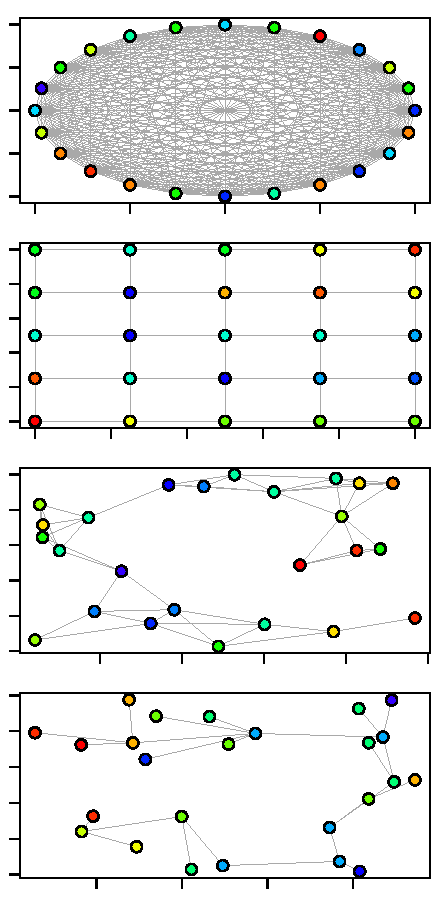
\includegraphics[width=0.3\textwidth]{Networks.pdf}
\end{figure}

\newpage

%------------------------
\subsection*{Figure 2}

\begin{figure}[ht!]
	\centering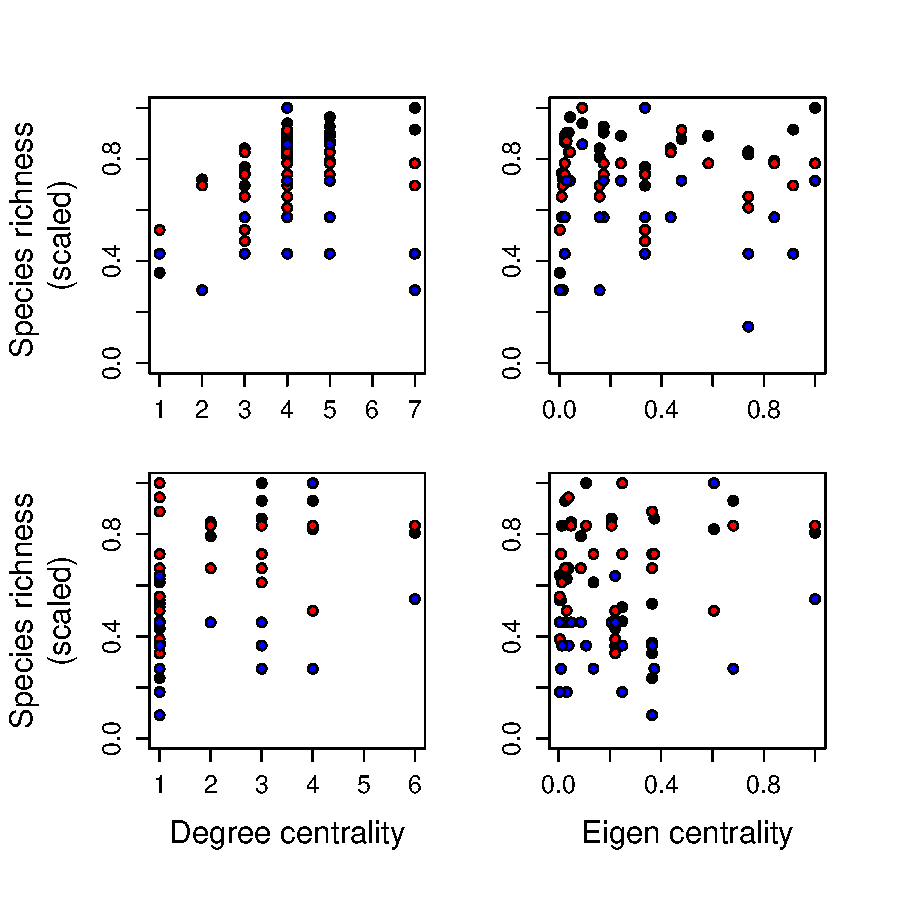
\includegraphics[width=0.75\textwidth]{Centrality.pdf}
\end{figure}

\newpage

%------------------------
\subsection*{Figure 3}

\begin{figure}[ht!]
	\centering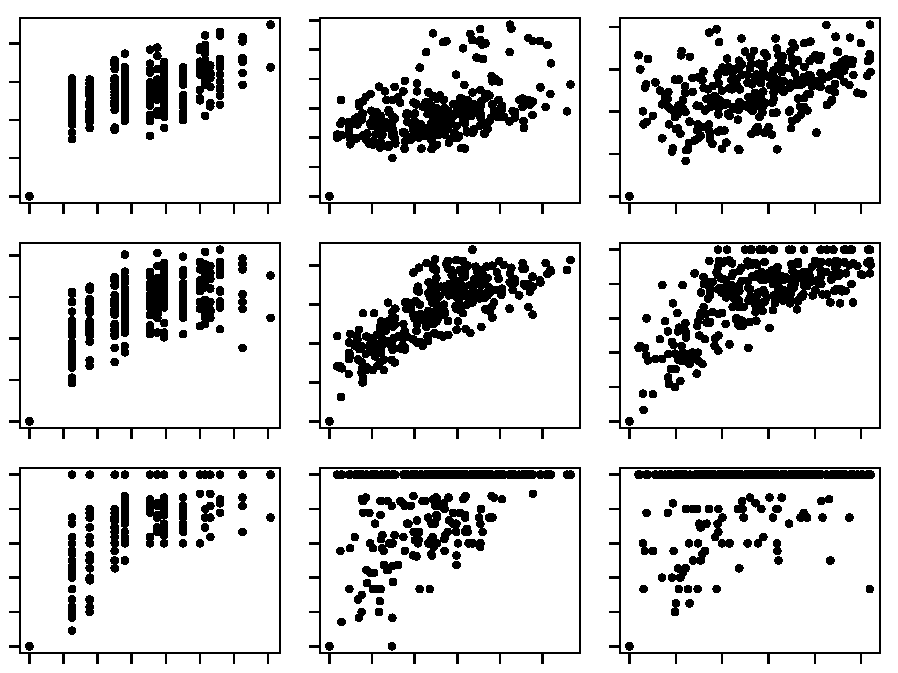
\includegraphics[width=0.65\textwidth]{BetaGeoDist.pdf}
\end{figure}

\newpage

%------------------------
\subsection*{Figure 4}

\begin{figure}[ht!]
	\centering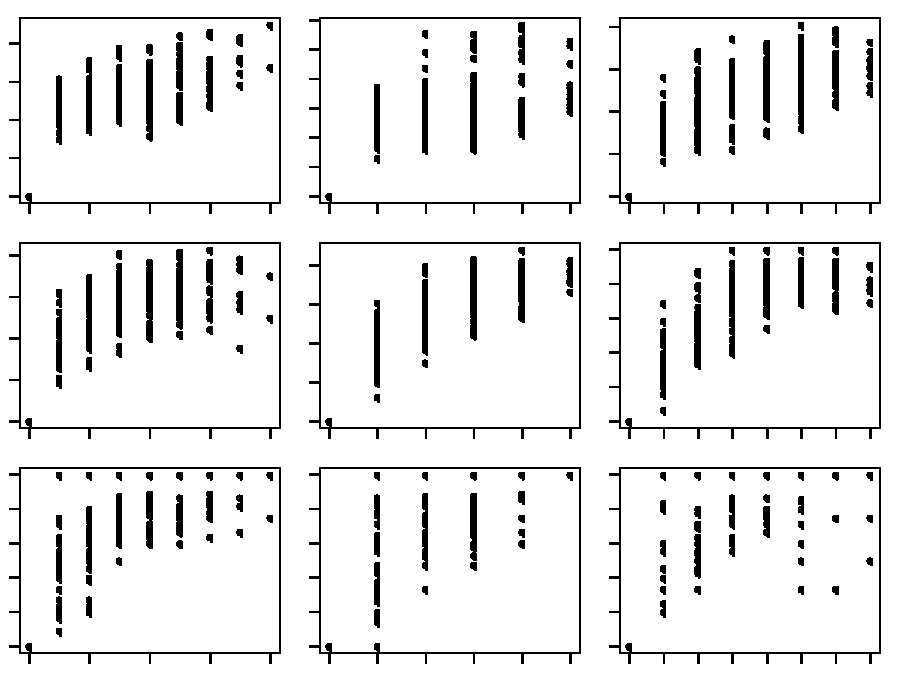
\includegraphics[width=0.65\textwidth]{BetaTopoDist.pdf}
\end{figure}

\newpage

\end{document}
%========================================================%
